\section{Segment routing formalization}

\label{section:sr-formal}

The starting point of our segment routing formalization is the concept of segment routing path, or sr-path for short.

\begin{definition}
Let $G$ be a network. A \emph{sr-path} $\sr{p}$ on $G$ is a sequence $\langle x_1, \ldots, x_l \rangle$ such that each $x_i \in V(G) \cup E(G)$.
%We use the notation $\sr{p}_i = x_i$ to represent the $i$-th element in the sequence.
\end{definition}

We represent sr-paths with the vector notation to be able to more easily distinguish between a path $p$ and a 
sr-path $\sr{p}$ in the network $G$. In practice, the elements of $\sr{p}$ that are nodes model node segments and
the elements of $\sr{p}$ that are edges model adjacency segments. It is important to understand that, because of ECMP, a sr-path
actually can correspond to a set of paths in the original network. 

Consider the sr-path $\sr{p} = \langle \node{a}, \node{c}, \node{e}, (\node{f}, \node{j}), \node{i} \rangle$ shown in
Figure \ref{fig:sr-path}. The solid green edges show the set of edges that belong to shortest paths between consecutive segments
and the dashed green edge represents the adjacency segment $(\node{f}, \node{j})$. The square boxes represent segments. The box is represented next to
a node for node segments and on top of the link of an adjacency segment. So, in this case, $x_1 = \node{a}, x_2 = \node{c}, x_3 = \node{e}, x_4 = \edge{f}{j}$
and $x_5 = \node{i}$.

In this example, between nodes \node{c} and \node{e} there are two shortest paths, namely
$((\node{c}, \node{d}), (\node{d}, \node{e}))$ and $((\node{c}, \node{b}), (\node{b}, \node{e}))$. In the same way,
two shortest paths exist between nodes \node{e} and \node{f} because we have two parallel links with the same IGP weight
between them. In each case, any of those two paths could be used to forward packets over this
sr-path. Thus, we see that the sr-path $\sr{p}$ can correspond to four paths over the original network, namely,

\begin{align*}
((\node{a}, \node{c}), (\node{c}, \node{d}), (\node{d}, \node{e}), (\node{e}, \node{f}, i_1), (\node{f}, \node{j}), (\node{j}, \node{h}), (\node{h}, \node{i})), \\
((\node{a}, \node{c}), (\node{c}, \node{d}), (\node{d}, \node{e}), (\node{e}, \node{f}, i_2), (\node{f}, \node{j}), (\node{j}, \node{h}), (\node{h}, \node{i})), \\
((\node{a}, \node{c}), (\node{c}, \node{b}), (\node{b}, \node{e}), (\node{e}, \node{f}, i_1), (\node{f}, \node{j}), (\node{j}, \node{h}), (\node{h}, \node{i})), \\
((\node{a}, \node{c}), (\node{c}, \node{b}), (\node{b}, \node{e}), (\node{e}, \node{f}, i_2), (\node{f}, \node{j}), (\node{j}, \node{h}), (\node{h}, \node{i})) \\
\end{align*}

where $(\node{e}, \node{f}, i_1)$ and $(\node{e}, \node{f}, i_2)$ represent the two links between $\node{e}$ and $\node{f}$.

\begin{figure}
\begin{center}
\begin{tikzpicture}
\def\x{0}
\def\y{0}
\node[scale=0.15] (a) at (0.5 + \x,  0.5 + \y) {\router{a}{marked}};
\node[scale=0.15] (b) at (0.5 + \x, -1.0 + \y) {\router{b}{router}};
\node[scale=0.15] (c) at (2.5 + \x,  0.0 + \y) {\router{c}{marked}};
\node[scale=0.15] (d) at (4.5 + \x,  0.0 + \y) {\router{d}{router}};
\node[scale=0.15] (e) at (4.0 + \x, -2.0 + \y) {\router{e}{marked}};
\node[scale=0.15] (g) at (6.0 + \x,  0.5 + \y) {\router{g}{router}};
\node[scale=0.15] (i) at (8.0 + \x,  0.0 + \y) {\router{i}{marked}};
\node[scale=0.15] (h) at (7.0 + \x, -1.5 + \y) {\router{h}{router}};
\node[scale=0.15] (f) at (4.0 + \x, -3.5 + \y) {\router{f}{router}};
\node[scale=0.15] (j) at (8.0 + \x, -2.5 + \y) {\router{j}{router}};
\draw[line width=2] (f) edge[above, sloped] node[black,font=\bfseries] {\tiny \texttt{}} (j);
\draw[line width=2] (h) edge[above, sloped] node[black,font=\bfseries] {\tiny \texttt{}} (j);
\draw[line width=2] (a) edge[above, sloped] node[black,font=\bfseries] {\tiny \texttt{}} (b);
\draw[line width=2] (b) edge[above, sloped] node[black,font=\bfseries] {\tiny \texttt{}} (c);
\draw[line width=2] (b) edge[above, sloped] node[black,font=\bfseries] {\tiny \texttt{}} (e);
\draw[line width=2] (b) edge[above, sloped] node[black,font=\bfseries] {\tiny \texttt{}} (f);
\draw[line width=2] (e) edge[above, sloped, bend left=10] node[black,font=\bfseries] {\tiny \texttt{}} (f);
\draw[line width=2] (e) edge[above, sloped, bend right=10] node[black,font=\bfseries] {\tiny \texttt{}} (f);
\draw[line width=2] (h) edge[above, sloped] node[black,font=\bfseries] {\tiny \texttt{}} (f);
\draw[line width=2] (g) edge[above, sloped] node[black,font=\bfseries] {\tiny \texttt{}} (i);
\draw[line width=2] (i) edge[above, sloped] node[black,font=\bfseries] {\tiny \texttt{}} (h);
\draw[line width=2]  (d) edge[above, sloped] node[black,font=\bfseries] {\tiny \texttt{}} (g);
\draw[line width=2]  (d) edge[above, sloped] node[black,font=\bfseries] {\tiny \texttt{}} (e);
\draw[line width=2]  (e) edge[above, sloped] node[black,font=\bfseries] {\tiny \texttt{}} (h);
\draw[line width=2]  (g) edge[above, sloped] node[black,font=\bfseries] {\tiny \texttt{}} (h);
\draw[line width=2]  (c) edge[above, sloped] node[black,font=\bfseries] {\tiny \texttt{}} (d);
\draw[line width=2]  (a) edge[above, sloped] node[black,font=\bfseries] {\tiny \texttt{}} (b);
\draw[line width=2]  (a) edge[above, sloped] node[black,font=\bfseries] {\tiny \texttt{}} (c);

%%%%
\draw (a) edge[line width=3, darkgreen, above, ->, bend left = 20] (c);
\draw (c) edge[line width=3, darkgreen, above, ->, bend right = 20] (d);
\draw (c) edge[line width=3, darkgreen, above, ->, bend right = 20] (b);
\draw (b) edge[line width=3, darkgreen, above, ->, bend left = 20] (e);
\draw (d) edge[line width=3, darkgreen, above, ->, bend right = 20] (e);

\draw (j) edge[line width=3, darkgreen, above, ->, bend left = 20] (h);
\draw (f) edge[line width=4, darkgreen, ->, dotted] node[line width = 1, draw, solid, black, fill=green] {\footnotesize $x_4$} (j);

\draw (h) edge[line width=3, darkgreen, above, ->, bend left = 20] (i);
\draw (e) edge[line width=3, darkgreen, above, ->, bend right = 30] (f);
\draw (e) edge[line width=3, darkgreen, above, ->, bend left = 30] (f);

\node[left = 0.1cm of a, draw, fill=green] {\footnotesize $x_1$};
\node[above = 0.1cm of c, draw, fill=green] {\footnotesize $x_2$};
\node[above right = 0.1cm of e, draw, fill=green] {\footnotesize $x_3$};
\node[right = 0.1cm of i, draw, fill=green] {\footnotesize $x_4$};

\end{tikzpicture}
\end{center}
\caption{Illustration of sr-path $\sr{p} = \langle \node{a}, \node{c}, \node{e}, (\node{f}, \node{j}), \node{i} \rangle$.}
\label{fig:sr-path}
\end{figure}


In general, when we use a sr-path $\sr{p} = \langle x_1, \ldots, x_l \rangle$ to forward traffic, between segments $x_i$ and $x_{i + 1}$ the set of paths
over which this traffic might be sent corresponds to the set of all shortest paths between those segments. In this thesis we consider two models for
forwarding traffic over ECMP:

\begin{enumerate}
 \item \emph{Hash model}: Whenever several next-hops exists with respect to the IGP shortest paths, a hash function is used to select which of them is used.
 This hash function is unknown and depends on the traffic that is sent. From a practical point of view this, more or less, corresponds to assuming that one of the
 multiple shortest paths is selected at random.
 
 \item \emph{Split model}: The traffic is split evenly between all shortest paths. This means that if, for instance, a router contains two next-hops, it will forward
 $50\%$ of the traffic towards one of them and the other $50\%$ towards the other.
\end{enumerate}


But these segments, $x_i$ and $x_{i + 1}$ might not both correspond to nodes in which case we need to give a precise definition of what the set of shortest paths between two segments means. 
In general, we have four cases which are summarized
in Figure \ref{fig:4case-sr}. If we have two node segments $x_i = v, x_{i + 1} = u$ then it is the subgraph between $v$ and $u$, $\sp(v, u)$. 
If $x_i = v$ and $x_{i + 1} = (u_1, u_2)$ then it the subgraph between $v$ and $u_1$, $\sp(v, u_1)$. If $x_i = (v_1, v_2)$ and $x_{i + 1} = u$ then it is
the shortest path subgraph between $v_2$ and $u$. Finally, if both are adjacency segments with $x_i = (v_1, v_2)$ and $x_{i + 1} = (u_1, u_2)$ then it is
$\sp(v_2, u_1)$.

\begin{figure}[H]
\begin{center}
\begin{tabular}{c}
\begin{tikzpicture}
\node[scale=0.15] (v) at (0, 0) {\router{$v$}{marked}};
\node[scale=0.15] (u) at (3, 0) {\router{$u$}{marked}};
\path (v) edge[line width=2, darkgreen, out=-30, in=240, wavy, ->] (u);
\path (v) edge[line width=2, darkgreen, out=30, in=150, wavy, ->] (u);
\node at (0, 1) {$x_i = v$};
\node at (3, 1) {$x_{i+1} = u$};
\node[darkgreen,font=\bfseries] at (1.5, 0) {$\sp(v, u)$};
\end{tikzpicture}
\\
\emph{Case 1:} $x_i$ and $x_{i + 1}$ are both node segments
\\[0.5cm]
\begin{tikzpicture}
\node[scale=0.15] (v) at (0, 0) {\router{$v$}{marked}};
\node[scale=0.15] (u1) at (3, 0) {\router{$u_1$}{router}};
\node[scale=0.15] (u2) at (5, 0) {\router{$u_2$}{router}};
\path (v) edge[line width=2, darkgreen, out=-30, in=240, wavy, ->] (u1);
\path (v) edge[line width=2, darkgreen, out=30, in=150, wavy, ->] (u1);
\draw[line width=2]  (u1) edge[above, sloped] node[black,font=\bfseries] (l) {} (u2);
\draw (u1) edge[line width=4, darkgreen, above, ->, dotted] (u2);
\node at (0, 1) {$x_i = v$};
\node at (4, 1) {$x_{i+1} = (u_1, u_2)$};
\node[darkgreen,font=\bfseries] at (1.5, 0) {$\sp(v, u_1)$};
\end{tikzpicture}
\\
\emph{Case 2:} $x_i$ is a node segment and $x_{i + 1}$ is an adjacency segment
\\[0.5cm]
\begin{tikzpicture}
\node[scale=0.15] (v1) at (0, 0) {\router{$v_1$}{router}};
\node[scale=0.15] (v2) at (2, 0) {\router{$v_2$}{router}};
\node[scale=0.15] (u) at (5, 0) {\router{$u$}{marked}};
\path (v2) edge[line width=2, darkgreen, out=-30, in=240, wavy, ->] (u);
\path (v2) edge[line width=2, darkgreen, out=30, in=150, wavy, ->] (u);
\draw[line width=2]  (v1) edge[above, sloped] node[black,font=\bfseries] (l) {} (v2);
\draw (v1) edge[line width=4, darkgreen, above, ->, dotted] (v2);
\node at (1, 1) {$x_i = (v_1, v_2)$};
\node at (5, 1) {$x_{i+1} = u$};
\node[darkgreen,font=\bfseries] at (3.5, 0) {$\sp(v_2, u)$};
\end{tikzpicture}
\\
\emph{Case 3:} $x_i$ is an adjacency segment and $x_{i + 1}$ is a node segment
\\[0.5cm]
\begin{tikzpicture}
\node[scale=0.15] (v1) at (0, 0) {\router{$v_1$}{router}};
\node[scale=0.15] (v2) at (2, 0) {\router{$v_2$}{router}};
\node[scale=0.15] (u1) at (5, 0) {\router{$u_1$}{router}};
\node[scale=0.15] (u2) at (7, 0) {\router{$u_2$}{router}};
\path (v2) edge[line width=2, darkgreen, out=-30, in=240, wavy, ->] (u1);
\path (v2) edge[line width=2, darkgreen, out=30, in=150, wavy, ->] (u1);
\draw[line width=2]  (v1) edge[above, sloped] node[black,font=\bfseries] (l) {} (v2);
\draw (v1) edge[line width=4, darkgreen, above, ->, dotted] (v2);
\draw[line width=2]  (u1) edge[above, sloped] node[black,font=\bfseries] (l) {} (u2);
\draw (u1) edge[line width=4, darkgreen, above, ->, dotted] (u2);
\node at (1, 1) {$x_i = (v_1, v_2)$};
\node at (6, 1) {$x_{i+1} = (u_1, u_2)$};
\node[darkgreen,font=\bfseries] at (3.5, 0) {$\sp(v_2, u_1)$};
\end{tikzpicture}
\\
\emph{Case 4:} $x_i$ and $x_{i + 1}$ are both adjacency segments
\end{tabular}
\end{center}
\caption{Shortest paths between consecutive segments.}
\label{fig:4case-sr}
\end{figure}

Having to deal with these four cases would be very cumbersome. When considering a sr-path $\sr{p}$ we want to have a way to
ignore as much as possible the nature of each of the segments. This will make proving results involving sr-paths easier and also
will ease the readability of proofs. This lead us to define the following notation so that we can
very simply capture all four cases.

\begin{definition}
Let $G$ be a network and $\sr{p} = \langle x_1, \ldots, x_l \rangle$. If $x_i \in V(G)$ we define $x^1_i = x^2_i = x_i$ and
if $x_i = (u_1, u_2) \in E(G)$ we define $x^1_i = u_1$ and $x^2_i = u_2$. 
\end{definition}

With this notation, we can now simply say that the set of shortest paths between two consecutive segments $x_i$ and $x_{i + 1}$
of a sr-path $\sr{p}$ is the subgraph $\sp(x^2_i, x^1_{i + 1})$. This works regardless of what the type of segments $x_i$ and $x_{i + 1}$
are. This notation also makes it easy to refer to the starting and ending routers of a sr-path.

\begin{definition}
Let $G$ be a network and $\sr{p} = \langle x_1, \ldots, x_l \rangle$. We say that $\sr{p}$ is a sr-path from node $x^1_1$ to
$x^2_l$. We say that $x^1_1$ is the first node of $\sr{p}$ and $x^2_l$ is the last node of $\sr{p}$. A sr-path that
starts and ends at the same node is called a sr-cycle.
\end{definition}

As we mentioned in the introduction of this chapter, when we use segment routing as a forwarding mechanism, we need to append to the packet 
header the segments that are to be used. Commercial routers have strong limitations regarding the size of this header. Some routers can
support sr-paths with up to $10$ segments but on average this number is closer to $5$ \cite{Tantsura_SID:2017}.
This means that it is important to be able to capture the cost, in terms of segments, of a sr-path. A node segment needs to contain
the IP address of the corresponding router whereas an adjacency segment needs the IP address of the source node of the corresponding link
as well as the interface identifier of that link. For this reason, we model the cost of individual segments and sr-paths as follows.

\begin{definition}
Let $G$ be a network and $\sr{p} = \langle x_1, \ldots x_l \rangle$ a sr-path on $G$. We define the cost of $x_i$ as
\[ \cost(x_i) =
  \begin{cases}
    1 & \quad \text{if } x_{i} \in V(G) \\
    2 & \quad \text{otherwise}
  \end{cases}
\]
We define the \emph{segment cost} of $\sr{p}$ as
$$
\cost(\sr{p}) = \sum_{i = 1}^l \cost(x_i)
$$
\end{definition}

Note that this model does not exactly match the reality. In practice, if the first segment is a node segment, its IP address will never be put into the
segment stack. Also, if the first segment is an adjacency segment only the link interface would be necessary
for the same reason. We chose to ignore this and count each segment equally because it greatly simplifies the mathematical developments. Furthermore, we
believe that the model is close enough that this will have a minor impact in practice. In the worst case, we overestimate the real segment cost
of a sr-path by $1$.

\begin{definition}
Let $G$ be a network. We denote the set of all sr-paths on $G$ by $\sr{\mathcal{P}}$. Given $k \in \mathbb{N}$ we define
$$
\mathcal{\sr{P}}_k(G) = \left\{ \sr{p} \mid \text{$\sr{p}$ is a sr-path on $G$ and $\cost(\sr{p}) \leq k$} \right\}.
$$
Finally, given $s, t \in V(G)$ we denote the set of all sr-paths from $s$ to $t$ of segment cost at most $k$
by $\Pk(s, t)$.

\end{definition}

We now define some operations on sr-paths and prove some of theirs properties.
 
\begin{definition}
Let $G$ be a network and $\sr{p} = \langle x_1, \ldots, x_l \rangle, \sr{q} = \langle y_1, \ldots, y_r \rangle$ be two sr-paths on $G$. We 
define the sum of $\sr{p}$ and $\sr{q}$ as
$$
\sr{p} + \sr{q} = \langle x_1, \ldots, x_l, y_1, \ldots, y_r \rangle
$$
\end{definition}

\begin{lemma}
\label{lemma:srsumcost}
Let $G$ be a network and $\sr{p} = \langle x_1, \ldots, x_l \rangle, \sr{q} = \langle y_1, \ldots, y_r \rangle$ be two sr-paths on $G$. Then
$$
\cost(\sr{p} + \sr{q}) = \cost(\sr{p}) + \cost(\sr{q}) 
$$
\end{lemma}

\begin{proof}
\begin{align*}
\cost(\sr{p} + \sr{q}) & = \cost(\langle x_1, \ldots, x_l, y_1, \ldots, y_r) \\
& = \sum_{i = 1}^l \cost(x_i) + \sum_{i = 1}^r \cost(y_i) \\
& = \cost(\sr{p}) + \cost(\sr{q})
\end{align*}
\end{proof}

Addition of sr-paths will turn out to be useful to prove
bounds on the segment cost of sr-paths produced by some of our algorithms. However, 
addition of sr-paths does not care about the segments contained in each path. It simply takes all segments
from both paths and put them in order into a single sr-path. For example, it could be the case that $x_l = y_1$
so the resulting sr-path would have a segment repeated twice next to each other. This does not 
cause any practical problem but in terms of routing it is redundant. Moreover, it wastes space in the segment stack. This can be the case even if $x_l \neq y_1$ but the last node of $x_l$ and the first node of $y_1$ 
are the same, that is, if $x^2_l = y^1_1$. For instance let $\sr{p} = \langle \node{a}, \node{f} \rangle$ and
$\sr{q} = \langle (\node{f}, \node{j}), \node{i} \rangle$. Then 
$\sr{p} + \sr{q} = \langle \node{a}, \node{f}, (\node{f}, \node{j}), \node{i} \rangle$. 
In terms of routing, this sr-path traverses the same links as the sr-path $\langle \node{a}, (\node{f}, \node{j}), \node{i} \rangle$
but it costs one more because it has a useless node segment on $\node{f}$.
With this in mind, we define a concatenation operation $\oplus$ on sr-paths which takes this into account and discards useless segments at the concatenation
point in the resulting sr-path.

% \begin{figure}[H]
% \begin{center}
% \begin{tikzpicture}
% \def\x{0}
% \def\y{0}
% \node[scale=0.15] (a) at (0.5 + \x,  0.5 + \y) {\router{a}{green}};
% \node[scale=0.15] (b) at (0.5 + \x, -1.0 + \y) {\router{b}{router}};
% \node[scale=0.15] (c) at (2.5 + \x,  0.0 + \y) {\router{c}{router}};
% \node[scale=0.15] (d) at (4.5 + \x,  0.0 + \y) {\router{d}{router}};
% \node[scale=0.15] (e) at (4.0 + \x, -2.0 + \y) {\router{e}{router}};
% \node[scale=0.15] (g) at (6.0 + \x,  0.5 + \y) {\router{g}{router}};
% \node[scale=0.15] (i) at (8.0 + \x,  0.0 + \y) {\router{i}{green}};
% \node[scale=0.15] (h) at (7.0 + \x, -1.5 + \y) {\router{h}{router}};
% \node[scale=0.15] (f) at (4.0 + \x, -3.5 + \y) {\router{f}{green}};
% \node[scale=0.15] (j) at (8.0 + \x, -2.5 + \y) {\router{j}{green}};
% \draw[line width=2] (f) edge[above, sloped] node[black,font=\bfseries] {\tiny \texttt{}} (j);
% \draw[line width=2] (h) edge[above, sloped] node[black,font=\bfseries] {\tiny \texttt{}} (j);
% \draw[line width=2] (a) edge[above, sloped] node[black,font=\bfseries] {\tiny \texttt{}} (b);
% \draw[line width=2] (b) edge[above, sloped] node[black,font=\bfseries] {\tiny \texttt{}} (c);
% \draw[line width=2] (b) edge[above, sloped] node[black,font=\bfseries] {\tiny \texttt{}} (e);
% \draw[line width=2] (b) edge[above, sloped] node[black,font=\bfseries] {\tiny \texttt{}} (f);
% \draw[line width=2] (e) edge[above, sloped, bend left=10] node[black,font=\bfseries] {\tiny \texttt{}} (f);
% \draw[line width=2] (e) edge[above, sloped, bend right=10] node[black,font=\bfseries] {\tiny \texttt{}} (f);
% \draw[line width=2] (h) edge[above, sloped] node[black,font=\bfseries] {\tiny \texttt{}} (f);
% \draw[line width=2] (g) edge[above, sloped] node[black,font=\bfseries] {\tiny \texttt{}} (i);
% \draw[line width=2] (i) edge[above, sloped] node[black,font=\bfseries] {\tiny \texttt{}} (h);
% \draw[line width=2]  (d) edge[above, sloped] node[black,font=\bfseries] {\tiny \texttt{}} (g);
% \draw[line width=2]  (d) edge[above, sloped] node[black,font=\bfseries] {\tiny \texttt{}} (e);
% \draw[line width=2]  (e) edge[above, sloped] node[black,font=\bfseries] {\tiny \texttt{}} (h);
% \draw[line width=2]  (g) edge[above, sloped] node[black,font=\bfseries] {\tiny \texttt{}} (h);
% \draw[line width=2]  (c) edge[above, sloped] node[black,font=\bfseries] {\tiny \texttt{}} (d);
% \draw[line width=2]  (a) edge[above, sloped] node[black,font=\bfseries] {\tiny \texttt{}} (b);
% \draw[line width=2]  (a) edge[above, sloped] node[black,font=\bfseries] {\tiny \texttt{}} (c);
% 
% %%%%
% \draw (a) edge[line width=3, darkgreen, above, ->, bend right = 20] (b);
% \draw (b) edge[line width=3, darkgreen, above, ->, bend right = 20] (f);
% 
% \draw (j) edge[line width=3, darkgreen, above, ->, bend left = 20] (h);
% \draw (f) edge[line width=4, darkgreen, above, ->, dotted] (j);
% 
% \draw (h) edge[line width=3, darkgreen, above, ->, bend left = 20] (i);
% 
% \end{tikzpicture}
% \end{center}
% \label{fig:sr-add}
% \caption{Illustration of sr-path $\sr{p} + \sr{q} = \langle \node{a}, \node{f} \rangle + \langle (\node{f}, \node{j}), \node{i} \rangle = \langle \node{a}, \node{f}, (\node{f}, \node{j}), \node{i} \rangle$.}
% \end{figure}

\begin{definition}
\label{def:sr-concat}
Let $G$ be a network and $\sr{p} = \langle x_1, \ldots, x_l \rangle$ be a sr-path from
$a$ to $b$ and $\sr{q} = \langle y_1, \ldots, y_r \rangle$ be a sr-path from $b$ to $c$, where $a, b, c \in V(G)$.
We  define the concatenation of $\sr{p}$ and $\sr{q}$ as
\[ \sr{p} \oplus \sr{q} =
  \begin{cases}
    \langle x_1, \ldots, x_l, y_2, \ldots, y_r \rangle & \quad \text{if } x_l = y_1 = b \in V(G) \\
    \langle x_1, \ldots, x_l, y_2, \ldots, y_r \rangle & \quad \text{if } x_l \in E(G) \text{ and } y_1 \in V(G) \\
    \langle x_1, \ldots, x_{l - 1}, y_1, \ldots, y_r \rangle & \quad \text{if } x_l \in V(G) \text{ and } y_1 \in E(G) \\
    \langle x_1, \ldots, x_l, y_1, \ldots, y_r \rangle & \quad \text{if } x_l \in E(G) \text{ and } y_1 \in E(G) \\
  \end{cases}
\]
\end{definition}

With sr-path concatenation we avoid consecutive redundant segments by removing them if necessary beforehand.
For the above example with $\sr{p} = \langle \node{a}, \node{f} \rangle$ and
$\sr{q} = \langle (\node{f}, \node{j}), \node{i} \rangle$ we have 
$\sr{p} \oplus \sr{q} = \langle \node{a}, (\node{f}, \node{j}), \node{i} \rangle$. Figure \ref{fig:sr-concat}
illustrates the four cases of sr-path concatenation from Definition \ref{def:sr-concat}.

\begin{figure}[H]
\begin{center}
\begin{tabular}{c}
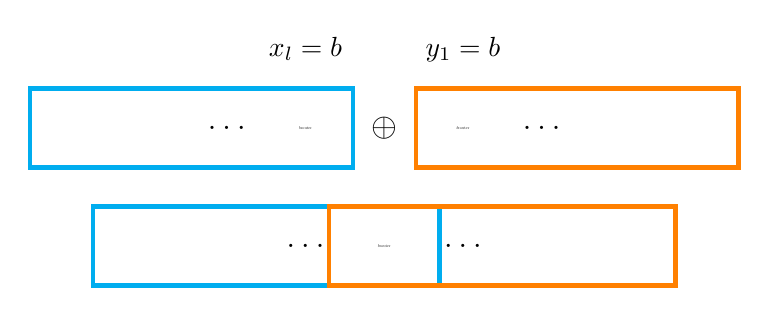
\begin{tikzpicture}
\draw[cyan, ultra thick] (-3.5, -0.5) rectangle (0.6, 0.5);
\draw[orange, ultra thick] (1.4, -0.5) rectangle (5.5, 0.5);

\node[scale=0.15] (v) at (0, 0) {\router{$b$}{router}};
\node[scale=0.15] (u) at (2, 0) {\router{$b$}{router}};
\node at (0, 1) {$x_l = b$};
\node at (2, 1) {$y_{1} = b$};
\node[left of=v] {\large $\ldots$};
\node[right of=u] {\large $\ldots$};

\node at (1, 0) {\large $\oplus$};
\node[rotate=-90] at (1, -0.75) {\large $\rightarrowtail$};

\node[scale=0.15] (b) at (1, -1.5) {\router{$b$}{router}};
\node[left of=b] {\large $\ldots$};
\node[right of=b] {\large $\ldots$};

\draw[cyan, ultra thick] (-2.7, -2) rectangle (1.7, -1);
\draw[orange, ultra thick] (0.3, -2) rectangle (4.7, -1);

\end{tikzpicture}
\\[0.25cm]
\emph{Case 1:} $x_l = y_1 = b \in V$
\\[1cm]
\begin{tikzpicture}
\draw[cyan, ultra thick] (-3.5, -0.5) rectangle (0.6, 0.5);
\draw[orange, ultra thick] (1.4, -0.5) rectangle (5.5, 0.5);

\node[scale=0.15] (v) at (0, 0) {\router{$b$}{router}};
\node[scale=0.15] (u1) at (2, 0) {\router{$b$}{router}};
\node[scale=0.15] (u2) at (4, 0) {\router{$*$}{router}};
\draw[line width=2]  (u1) edge[above, sloped] node[black,font=\bfseries] (l) {} (u2);
\draw (u1) edge[line width=4, darkgreen, above, ->, dotted] (u2);
\node at (0, 1) {$x_l = b$};
\node at (3, 1) {$y_1 = (b, *)$};
\node at (1, 0) {\large $\oplus$};

\node[left of=v] {\large $\ldots$};
\node[right of=u2] {\large $\ldots$};
\node[rotate=-90] at (3, -0.75) {\large $\rightarrowtail$};

\node[scale=0.15] (x) at (3, -1.5) {\router{$*$}{router}};
\node[scale=0.15] (b) at (1, -1.5) {\router{$b$}{router}};
\node[left of=b] {\large $\ldots$};
\node[right of=x] {\large $\ldots$};
\draw[line width=2] (b) edge[above, sloped] (x);
\draw (b) edge[line width=4, darkgreen, above, ->, dotted] (x);

\draw[cyan, ultra thick] (-2.7, -2) rectangle (1.7, -1);
\draw[orange, ultra thick] (0.3, -2) rectangle (4.7, -1);

\end{tikzpicture}
\\[0.25cm]
\emph{Case 2:} $x_l \in E(G)$, $y_{1} \in V(G)$ and $x^2_l =  y_1 = b$
\\[1cm]
\begin{tikzpicture}
\draw[cyan, ultra thick] (-1.5, -0.5) rectangle (2.6, 0.5);
\draw[orange, ultra thick] (3.4, -0.5) rectangle (7.5, 0.5);

\node[scale=0.15] (v1) at (0, 0) {\router{$x$}{router}};
\node[scale=0.15] (v2) at (2, 0) {\router{$b$}{router}};
\node[scale=0.15] (u) at (4, 0) {\router{$b$}{router}};
\draw[line width=2]  (v1) edge[above, sloped] node[black,font=\bfseries] (l) {} (v2);
\draw (v1) edge[line width=4, darkgreen, above, ->, dotted] (v2);
\node at (1, 1) {$x_l = (*, b)$};
\node at (4, 1) {$y_1 = b$};
\node at (3, 0) {\large $\oplus$};

\node[left of=v1] {\large $\ldots$};
\node[right of=u] {\large $\ldots$};
\node[rotate=-90] at (3, -0.75) {\large $\rightarrowtail$};

\node[scale=0.15] (x) at (1, -1.5) {\router{$x$}{router}};
\node[scale=0.15] (b) at (3, -1.5) {\router{$b$}{router}};
\node[left of=x] {\large $\ldots$};
\node[right of=b] {\large $\ldots$};
\draw[line width=2] (x) edge[above, sloped] (b);
\draw (x) edge[line width=4, darkgreen, above, ->, dotted] (b);
\draw[cyan, ultra thick] (-0.5, -2) rectangle (3.7, -1);
\draw[orange, ultra thick] (2.3, -2) rectangle (6.5, -1);

\end{tikzpicture}
\\[0.25cm]
\emph{Case 3:} $x_l \in V(G)$, $y_1 \in E(G)$ and $x_l = y^1_1 = b$
\\[1cm]
\begin{tikzpicture}
\draw[cyan, ultra thick] (-1.5, -0.5) rectangle (2.6, 0.5);
\draw[orange, ultra thick] (3.4, -0.5) rectangle (7.5, 0.5);

\node[scale=0.15] (v1) at (0, 0) {\router{$*$}{router}};
\node[scale=0.15] (v2) at (2, 0) {\router{$b$}{router}};
\node[scale=0.15] (u1) at (4, 0) {\router{$b$}{router}};
\node[scale=0.15] (u2) at (6, 0) {\router{$*$}{router}};
\draw[line width=2]  (v1) edge[above, sloped] node[black,font=\bfseries] (l) {} (v2);
\draw (v1) edge[line width=4, darkgreen, above, ->, dotted] (v2);
\draw[line width=2]  (u1) edge[above, sloped] node[black,font=\bfseries] (l) {} (u2);
\draw (u1) edge[line width=4, darkgreen, above, ->, dotted] (u2);
\node at (1, 1) {$x_l = (*, b)$};
\node at (5, 1) {$y_1 = (b, *)$};
\node at (3, 0) {\large $\oplus$};
\node[left of=v1] {\large $\ldots$};
\node[right of=u2] {\large $\ldots$};

\node[rotate=-90] at (3, -0.75) {\large $\rightarrowtail$};

\node[scale=0.15] (x) at (1, -1.5) {\router{$*$}{router}};
\node[scale=0.15] (b) at (3, -1.5) {\router{$b$}{router}};
\node[scale=0.15] (y) at (5, -1.5) {\router{$*$}{router}};
\node[left of=x] {\large $\ldots$};
\node[right of=y] {\large $\ldots$};
\draw[line width=2] (x) edge[above, sloped] (b);
\draw[line width=2] (b) edge[above, sloped] (y);
\draw (x) edge[line width=4, darkgreen, above, ->, dotted] (b);
\draw (b) edge[line width=4, darkgreen, above, ->, dotted] (y);

\draw[cyan, ultra thick] (-0.5, -2) rectangle (3.7, -1);
\draw[orange, ultra thick] (2.3, -2) rectangle (6.5, -1);


\end{tikzpicture}
\\[0.25cm]
\emph{Case 4:} $x_l \in E(G)$, $y_1 \in E(G)$ and $x^2_l = y^1_1 = b$
\end{tabular}
\end{center}
\caption{The four cases of sr-path concatenation.}
\label{fig:sr-concat}
\end{figure}

In contrast with sr-path addition, the cost of the resulting sr-path after a concatenation
will depend on the types of the segments at the end of the first path and at the start 
of the second.

\begin{lemma}
\label{lemma:concat-cost}
Let $G$ be a network and $\sr{p} = \langle x_1, \ldots, x_l \rangle$ be a sr-path from
$a$ to $b$ and $\sr{q} = \langle y_1, \ldots, y_r \rangle$ be a sr-path from $b$ to $c$, where $a, b, c \in V(G)$.
Then
\[ \cost(\sr{p} \oplus \sr{q}) =
  \begin{cases}
    \cost(\sr{p}) + \cost(\sr{q}) & \quad \text{if } x_l \in E(G) \text{ and } y_1 \in E(G) \\
    \cost(\sr{p}) + \cost(\sr{q}) - 1 & \quad \text{otherwise} \\
  \end{cases}
\]
\end{lemma}

\begin{proof}
If $x_l \in E(G)$ and $y_1 \in E(G)$ then $\sr{p} \oplus \sr{q} = \sr{p} + \sr{q}$ so the result comes from 
Lemma \ref{lemma:srsumcost}. Otherwise, in each case $\sr{p} \oplus \sr{q}$ has the same elements as $\sr{p} + \sr{q}$ except
that we removed a node segment with cost $1$. Thus, by Lemma \ref{lemma:srsumcost}, we have that
$$
\cost(\sr{p} \oplus \sr{q}) = \cost(\sr{p} + \sr{q}) - 1 = \cost(\sr{p}) + \cost(\sr{q}) - 1
$$
\end{proof}

These operations will be important later on because a lot of algorithms for solving problems related to segment routing
can be expressed as dynamic programs where the solution sr-path is built upon smaller sr-paths. These properties tell
use how the segment cost of the paths is affected by these operations.

It is often useful to refer to the set of nodes and edges that belong to some path represented by a sr-path leading
to the following definition.

\begin{definition}
Let $G$ be a network and $\sr{p} = \langle x_1, \ldots, x_l \rangle$ a sr-path on $G$. We define the set of nodes in $\sr{p}$ as
$$
V(\sr{p}) = \bigcup_{i = 1}^l \{x^1_i, x^2_i \} \quad \cup \quad \bigcup_{i = 2}^l V(\sp(x^2_{i - 1}, x^1_i))
$$
We define the set of edges of $\sr{p}$ as
$$
E(\sr{p}) = \left\{ x_i \mid \textrm{$x_i$ is an adjacency segment} \right\} \quad \cup \quad \bigcup_{i = 2}^l E(\sp(x^2_{i - 1}, x^1_i))
$$
\end{definition}

\begin{definition}
Let $G$ be a network and $\sr{p}$ be a sr-path on $G$. We call the subgraph $(V(G), E(\sr{p}))$ the \emph{forwarding
subnetwork} of $\sr{p}$ and denote it by $\forw(\sr{p})$. We write the set of edge in the forwarding graph as
$E(\forw(\sr{p})) = E(\sr{p})$. We can easily see that if $\sr{p} = \langle x_1, \ldots, x_l \rangle$ then
$$
E(\sr{p}) = \bigcup_{i = 2} E(\sp(x^2_{i - 1}, x^1_i)) \cup \bigcup{i : x_i \in E(G)} x_i.
$$
\end{definition}

To lighten the notation, we often omit the parenthesis and write $\forw \langle x_1, \ldots, x_l \rangle$ rather than
$\forw(\langle x_1, \ldots, x_l \rangle)$.

The forwarding subnetwork of a sr-path $\sr{p}$ encodes every path on which packets might travel when forwarded over $\sr{p}$.
However it does not encode how many times a given link is traversed by the sr-path because each edge that is traversed by $\sr{p}$ 
appears exactly once.

\begin{definition}
Let $G$ be a network and $\sr{p} = \langle x_1, \ldots, x_l \rangle$ be a sr-path on $G$. We say that $\sr{p}$ is \emph{deterministic} if and only if
for each $i \in \{2, \ldots, l\}$, there exists a unique shortest path between $x^2_{i - 1}$ and $x^1_i$.
\end{definition}

Deterministic sr-paths are important when we want to have guarantees about the set of links that are traversed
when one uses SR to forward traffic over a given sr-path. Because there exists a single shortest path between any two consecutive endpoints,
they never use ECMP. For this reason they map back to a unique path on the network $G$. This kind of paths will be important in Chapter \ref{chapter:scmon}
where we design an algorithm that leverages segment routing to provide network monitoring for detecting single link failures. In this context,
we will need to know exactly which links are covered by each sr-path used for the monitoring.

Another application of deterministic sr-paths, which we will tackle in the next section, is the reverse problem, where we start from a path on $G$
and we want to find a sr-path whose forwarding graph matches that path.

\begin{lemma}
\label{lemma:deterministic-concat}
Let $G$ be a network and $\sr{p}$ be a deterministic sr-path from
$a$ to $b$ and $\sr{q}$ be a deterministic sr-path from $b$ to $c$ 
then $\sr{p} \oplus \sr{q}$ is a deterministic sr-path
from $a$ to $c$.
\end{lemma}

\begin{proof}
The fact that $\sr{p} \oplus \sr{q}$ is well defined is simply because we assumed
that $\sr{p}$ is a sr-path from $a$ to $b$ and $\sr{q}$ a sr-path from $b$ to $c$. 
It remains to show that it is deterministic.

Write $\sr{p} = \langle x_1, \ldots, x_l \rangle$ and 
$\sr{q} = \langle y_1, \ldots, y_r \rangle$.
Let $z_i, z_{i + 1}$ be consecutive elements of $\sr{p} \oplus \sr{q}$. 
We need to prove that
there exists a unique shortest path between $z^2_i$ and $z^1_{i + 1}$.
If both $z_i, z_{i + 1}$ belong to $\sr{p}$ or $\sr{q}$ then this is true since both
$\sr{p}$ and $\sr{q}$ are deterministic. Otherwise, there are four cases that we need
to consider.

\emph{Case 1:} $x_l = y_1$ are both node segments. In this case we know that
$\sr{p} \oplus \sr{q} = \langle x_1, \ldots, x_l, y_2, \ldots, y_r \rangle$.
Thus, $z_i = x_l = y_1$ and $z_{i + 1} = y_2$. Hence, since $\sr{q}$ is deterministic,
there exists a unique shortest path between $z^2_i = y^2_1$ and $z^1_{i + 1} = y^1_2$.

\emph{Case 2:} $x_l,  y_1$ are both adjacency segments and 
$x^2_l = y^1_1$. In this case we know that
$\sr{p} \oplus \sr{q} = \langle x_1, \ldots, x_l, y_1, y_2, \ldots, y_r \rangle$.
Hence, $z_i = x_l$ and $z_{i + 1} = y_1$ so $z^2_i = x^2_l = y^1_1 = z^1_{i + 1}$ so
the unique shortest path between $z^2_i$ and $z^1_{i + 1}$ is the empty path.

\emph{Case 3:} $x_l$ is an adjacency segment and $y_1$ is a node segment such that
$x^2_l = y_1$. By definition, 
$\sr{p} \oplus \sr{q} = \langle x_1, \ldots, x_l, y_2, \ldots, y_r \rangle$.
Thus, $z_i = x_l$ and $z_{i + 1} = y_2$. Thus, since $\sr{q}$ is deterministic,
there exists a unique shortest path between $z^2_i = x^2_l = y^2_1$ and $z^1_{i + 1} = y^1_2$.

\emph{Case 4:} $x_l$ is a node segment and $y_1$ is an adjacent segment such that
$y^1_1 = x_l$. Therefore $\sr{p} \oplus \sr{q} = \langle x_1, \ldots, x_{l - 1}, y_1, y_2, \ldots, y_r \rangle$.
Thus, $z_i = x_{l - 1}$ and $z_{i + 1} = y_1$. Thus, since $\sr{p}$ is deterministic,
there exists a unique shortest path between $z^2_i = x^2_{l - 1}$ and $z^1_{i + 1} = y^1_2 = x^1_l$.
\end{proof}

\section{Acyclic sr-paths}
\label{section:acyclic}

Sr-paths can contain cycles as shown in Figure \ref{fig:cyclicsr}. In some situations we can take advantage of these
cycles to obtain better solution. We discuss one such example when we talk about traffic engineering in Chapter \ref{chapter:te}. 
In other situations we can show that cycles can never lead to an optimal solution.
We are now going to prove that we can always transform a sr-path that contains cycles into a sr-path that is acyclic,
visits a subset of the edges previously visited and does not have a higher segment cost. 
In the case of Figure \ref{fig:cyclicsr} we could achieve this by replacing node segment $\node{d}$ by $\node{e}$.
The set of edges in $\forw \langle \node{a}, \node{b}, \node{e}, \node{f} \rangle$ is a subset of the set of edges 
in $\forw \langle \node{a}, \node{b}, \node{d}, \node{f} \rangle$ but $\langle \node{a}, \node{b}, \node{e}, \node{f} \rangle$
is acyclic.

\begin{figure}[H]
\begin{center}
\begin{tikzpicture}
\def\x{0}
\def\y{0}
\node[scale=0.15] (a) at (0.5 + \x,  0.5 + \y) {\router{a}{marked}};
\node[scale=0.15] (b) at (0.5 + \x, -1.0 + \y) {\router{b}{marked}};
\node[scale=0.15] (c) at (2.5 + \x,  0.0 + \y) {\router{c}{router}};
\node[scale=0.15] (d) at (4.5 + \x,  0.0 + \y) {\router{d}{marked}};
\node[scale=0.15] (e) at (4.0 + \x, -2.0 + \y) {\router{e}{router}};
\node[scale=0.15] (g) at (6.0 + \x,  0.5 + \y) {\router{g}{router}};
\node[scale=0.15] (i) at (8.0 + \x,  0.0 + \y) {\router{i}{router}};
\node[scale=0.15] (h) at (7.0 + \x, -1.5 + \y) {\router{h}{router}};
\node[scale=0.15] (f) at (4.0 + \x, -3.5 + \y) {\router{f}{marked}};
\node[scale=0.15] (j) at (8.0 + \x, -2.5 + \y) {\router{j}{router}};
\draw[line width=2] (f) edge[above, sloped] node[black,font=\bfseries] {\tiny \texttt{}} (j);
\draw[line width=2] (h) edge[above, sloped] node[black,font=\bfseries] {\tiny \texttt{}} (j);
\draw[line width=2] (a) edge[above, sloped] node[black,font=\bfseries] {\tiny \texttt{}} (b);
\draw[line width=2] (b) edge[above, sloped] node[black,font=\bfseries] {\tiny \texttt{}} (c);
\draw[line width=2] (b) edge[above, sloped] node[black,font=\bfseries] {\tiny \texttt{}} (e);
\draw[line width=2] (b) edge[above, sloped] node[black,font=\bfseries] {\tiny \texttt{}} (f);
\draw[line width=2] (e) edge[above, sloped, bend left=10] node[black,font=\bfseries] {\tiny \texttt{}} (f);
\draw[line width=2] (e) edge[above, sloped, bend right=10] node[black,font=\bfseries] {\tiny \texttt{}} (f);
\draw[line width=2] (h) edge[above, sloped] node[black,font=\bfseries] {\tiny \texttt{}} (f);
\draw[line width=2] (g) edge[above, sloped] node[black,font=\bfseries] {\tiny \texttt{}} (i);
\draw[line width=2] (i) edge[above, sloped] node[black,font=\bfseries] {\tiny \texttt{}} (h);
\draw[line width=2]  (d) edge[above, sloped] node[black,font=\bfseries] {\tiny \texttt{}} (g);
\draw[line width=2]  (d) edge[above, sloped] node[black,font=\bfseries] {\tiny \texttt{}} (e);
\draw[line width=2]  (e) edge[above, sloped] node[black,font=\bfseries] {\tiny \texttt{}} (h);
\draw[line width=2]  (g) edge[above, sloped] node[black,font=\bfseries] {\tiny \texttt{}} (h);
\draw[line width=2]  (c) edge[above, sloped] node[black,font=\bfseries] {\tiny \texttt{}} (d);
\draw[line width=2]  (a) edge[above, sloped] node[black,font=\bfseries] {\tiny \texttt{}} (b);
\draw[line width=2]  (a) edge[above, sloped] node[black,font=\bfseries] {\tiny \texttt{}} (c);

%%%%
\draw (a) edge[line width=3, darkgreen, above, ->, bend right = 10] (b);
\draw (b) edge[line width=3, darkgreen, above, ->, bend right = 10] (c);
\draw (b) edge[line width=3, darkgreen, above, ->, bend left = 10] (e);
\draw (c) edge[line width=3, darkgreen, above, ->, bend right = 10] (d);
\draw (e) edge[line width=3, darkgreen, above, ->, bend right = 20] (d);
\draw (d) edge[line width=3, darkgreen, above, ->, bend right = 20] (e);
\draw (e) edge[line width=3, darkgreen, above, ->, bend left = 20] (f);
\draw (e) edge[line width=3, darkgreen, above, ->, bend right = 20] (f);

\draw (a) edge[line width=3, orange, above, ->, bend left = 10] (b);
\draw (b) edge[line width=3, orange, above, ->, bend left = 10] (e);

\draw (e) edge[line width=3, orange, above, ->, bend left = 40] (f);
\draw (e) edge[line width=3, orange, above, ->, bend right = 40] (f);



\node[left = 0.1cm of a, draw, fill=green] (x1) {\footnotesize $x_1$};
\node[left = 0.1cm of b, draw, fill=green] (x2) {\footnotesize $x_2$};
\node[above = 0.1cm of d, draw, fill=green] (x3) {\footnotesize $x_3$};
\node[below = 0.1cm of f, draw, fill=green] (x4) {\footnotesize $x_4$};

\node[left = 0.1cm of x1, draw, fill=orange!20!white] (y1) {\footnotesize $y_1$};
\node[left = 0.1cm of x2, draw, fill=orange!20!white] (y2) {\footnotesize $y_2$};
\node[left bottom = 0.1cm of e, draw, fill=orange!20!white] (y3) {\footnotesize $y_3$};
\node[left = 0.1cm of x4, draw, fill=orange!20!white] (y4) {\footnotesize $y_4$};

\end{tikzpicture}
\end{center}
\caption{Illustration of a cyclic sr-path $\sr{p} = \langle \node{a}, \node{b}, \node{d}, \node{f} \rangle$. It contains
cycle $(\edge{d}{e}, \edge{e}{d})$. The sr-path $\sr{q} = \langle \node{a}, \node{b}, \node{e}, \node{f} \rangle$ also goes
from $\node{a}$ to $\node{f}$ but is acyclic. It visits a subset of the edges of $\forw(\sr{p})$ so it is a sr-subpath
of $\sr{q}$.}
\label{fig:cyclicsr}
\end{figure}

Next we give a formal definition of cyclic sr-paths. 

\begin{definition}
Let $G$ be a network and $\sr{p}$ a sr-path on $G$. We say that $\sr{p}$ is \emph{cyclic} if $\forw(\sr{p})$ is
cyclic.
\end{definition}

Do not confuse this definition with sr-cycles. A sr-cycle is simply a sr-path whose first and last nodes are the same.
Of course any sr-cycle is cyclic. But not all cyclic sr-paths are sr-cycles. We start by proving the theorem in the case
where the sr-path contains only node segments.

The following simple lemma shows that if two nodes are connected then we can always find an acyclic sr-path between them.

\begin{lemma}
Let $G$ be a network and $u, v \in G$. If there exists a path from $u$ to $v$ on $G$ then there exists an acyclic sr-path
from $u$ to $v$.
\end{lemma}

\begin{proof}
We can simply take a minimal segmentation $\sr{p}$ of $p$. In this case $\forw(\sr{p}) = p$ so it is acyclic.
\end{proof}

\begin{definition}
Let $G$ be a network and $\sr{p}$ a sr-path from $u$ to $v$ on $G$. We say that $\sr{q}$ is a \emph{sr-subpath} of $\sr{p}$ if 
$\sr{q}$ is a sr-path from $u$ to $v$ and $\forw(\sr{q})$ is a subnetwork of $\forw(\sr{p})$.
\end{definition}

The next theorem shows that for any sr-path, we can always find a sr-subpath of it that is acyclic and whose segment
cost is at most the segment cost of the original path. This theorem has important practical implications as we will
see in Chapter \ref{chapter:disjoint}.

\begin{theorem}
\label{thm:sracyclic_noadj}
Let $G$ be a network with $\igp(e) > 0$ for all $e \in E(G)$, $u, v \in V(G)$ with $u \neq v$ and $\sr{p}$ be a sr-path on $G$ from $u$ to $v$ using only node segments. 
Then there exists an acyclic sr-path $\sr{q}$ from $u$ to $v$
such that $\forw(\sr{q}) \subseteq \forw(\sr{p})$ and $\cost(\sr{q}) \leq \cost(\sr{p})$.
\end{theorem}

\begin{proof}
Let $\sr{p} = \langle x_1, \ldots, x_n \rangle$. The proof is by induction on $n$. If $n = 1$
then $\forw(\sr{p})$ has 0 edges and is therefore acyclic. If $n = 2$ then $\forw(\sr{p})$ is equal to the
union of shortest paths from $x_1$ to $x_2$ which form an acyclic graph.
Assume that $\langle x_1, \ldots, x_{n - 1} \rangle$ is acyclic but $\sr{p}$ is not. We will show
how to construct $\sr{q}$ satisfying the theorem conditions.

Since $\sr{p}$ is cyclic, we can let $i$ be the smallest index such that
there exists a node $v$ in $\forw \langle x_i, x_{i + 1} \rangle$ that belongs to a cycle in $\forw(\sr{p})$.
If several such nodes exist, assume that $v$ is the one closest to $x_i$ (in terms of IGP, if several exist, choose any).

Let $\sr{q} = \langle x_1, \ldots, x_i, v, x_n\rangle$. Since $v$ belongs to both $\forw \langle x_i, x_{i + 1} \rangle$ and
$\forw \langle x_{n - 1}, x_n \rangle$ we have
$$
\forw \langle x_1, \ldots, x_i, v \rangle \subseteq \forw \langle x_1, \ldots, x_i, x_{i + 1} \rangle
$$
and
$$
\forw \langle v, x_n \rangle \subseteq \forw \langle x_{n - 1}, x_n \rangle
$$
so that
\begin{align*}
\forw(\sr{q}) & = \forw \langle x_1, \ldots, x_i, v \rangle \cup \forw \langle v, x_n \rangle \\
              & \subseteq \forw \langle x_1, \ldots, x_i, x_{i + 1} \rangle \cup \forw \langle x_{n - 1}, x_n \rangle \\
              & \subseteq \forw \langle x_1, \ldots, x_i, x_{i + 1} \rangle \cup \forw \langle x_{i + 2}, \ldots x_{n - 2} \rangle \cup \forw \langle x_{n - 1}, x_n \rangle \\
              & = \forw(\sr{p}).
\end{align*}
Similarly, we have
\begin{align*}
\cost(\sr{q}) & = \cost \langle x_1, \ldots, x_i, v \rangle + \cost \langle v, x_n \rangle - 1 \\
              & = \cost \langle x_1, \ldots, x_i, x_{i + 1} \rangle + \cost \langle x_{n - 1}, x_n \rangle - 1 \\
              & < \cost \langle x_1, \ldots, x_i, x_{i + 1} \rangle + \cost \langle x_{i + 2}, \ldots x_{n - 2} \rangle + \cost \langle x_{n - 1}, x_n \rangle \\
              & = \cost(\sr{p}).
\end{align*}
The sr-path $\sr{q}$ starts at $x_1 = u$ and ends at $x_n = v$. If $\sr{q}$ is acyclic then the proof is complete. Otherwise, let $c$
by a cycle on $\forw(\sr{q})$. Since both $\forw \langle x_1, \ldots, x_i, v \rangle$ and $\forw \langle v, x_n \rangle$ are acyclic,
$c$ cannot be fully contained in either one of them. This means that there must be a node $u \in V(c) \setminus v$ in 
$\forw \langle x_1, \ldots, x_i, v \rangle$. By choice of $v$, the distance from $x_i$ to $u$ and $v$ must be the same and $u$ must be
in the shortest path from $x_i$ to $v$. This is impossible since we assume that $\igp(e) > 0$ for all $e \in E(G)$.
\end{proof}

The theorem is also true in the general case where we allow the sr-path $\sr{p}$ to contain adjacency segments. However the proof is
quite tedious as it involves a lot of cases. Rather than provide a detailed proof, we instead provide the case analysis and a valid
acyclic sr-subpath in each case.

The construction works very similarly as in the proof of Theorem \ref{thm:sracyclic_noadj}. Let's focus on the general case
only. Assume that $\sr{p} = \langle x_1, \ldots, x_n \rangle$ is cyclic but $\langle x_1, \ldots, x_{n - 1} \rangle$ is acyclic. 
As in the above proof, let $i$ be the smallest index such that
there exists a node $v$ in $\forw \langle x_i, x_{i + 1} \rangle$ that belongs to a cycle in $\forw(\sr{p})$.
If several such nodes exist, assume that $v$ is the one closest to $x_i$ (in terms of IGP, if several exist, choose any).

With this choice of $x_i$ and $v$ we can build $\sr{q}$ by following Table \ref{tab:cases}. The construction of $\sr{q}$ depends on
two things:

\begin{enumerate}
 \item Where $v$ is crossed when we move on $\sr{p}$ from $x_i$ to $x_{i + 1}$.
 \item Where $v$ is crossed when we move on $\sr{p}$ from $x_{n - 1}$ to $x_n$.
\end{enumerate}

For the first, we consider three cases: (1) $v$ is the node $x^1_i$, (2) $v$ is the node $x^2_{i}$ or (3) $v$ is neither
of those nodes and belongs to a shortest path from $x^2_i$ to $x^1_{i + 1}$ (we represent this by $v \in \langle x^2_i, x^1_{i + 1} \rangle$
on the table). This is represented the columns of the table.

For the second, we consider five cases: (1) $v$ is the node $x^1_{n - 1}$, (2) $v$ is the node $x^2_{n - 1}$, (3) $v$ is the node $x^1_n$, 
(4) $v$ is the node $x^2_n$ and finally (5) $v$ is neither of those nodes and belongs the shortest path between $x^2_{n - 1}$ to $x^1_n$ 
(we represent this by $v \in \langle x^2_{n - 1}, x^1_n\rangle$ on the table). These cases are represented by the rows of the table.

For example, if $v = x^2_i$ and $v \in \langle x_{n - 1}, x_, \rangle$ then $\sr{q} = \langle x_1, \ldots, x_i, x_n \rangle$ is a 
solution.

Note that for construction to be correct we do not need to assume anything about the kind of segments $x_i$, $x_{i + 1}$, $x_{n-1}$ and
$x_n$ are. It may seem that we are assuming that they are adjacency segments but if they are not the construction still works. The only
thing that might happen is that we may have some repeated redundant segments in $\sr{q}$. However even with these, we can show that 
$\cost(\sr{q}) \leq \cost(\sr{p})$.

\begin{center}
\begin{table}
\footnotesize
\begin{tabular}{c|ccccc}
                                       & $v = x^1_i$ & $v = x^2_i$ & $v \in \langle x^2_i, x^1_{i + 1} \rangle$ \\[0.1cm]
                                       \midrule
$v = x^1_{n - 1}$                      & $\langle x_1, \ldots, x_{i-1}, x_{n - 1}, x_n \rangle$ 
                                       & $\langle x_1, \ldots, x_i, x_{n - 1}, x_n \rangle$ 
                                       & $\langle x_1, \ldots, x_i, x_{n - 1}, x_n \rangle$      \\[0.05cm]
                                       
$v = x^2_{n - 1}$                      & $\langle x_1, \ldots, x_{i-1}, v, x_n \rangle$ 
                                       & $\langle x_1, \ldots, x_{i}, x_n \rangle$ 
                                       & $\langle x_1, \ldots, x_{i}, v, x_n \rangle$    \\[0.05cm]
                                       
                                       
$v = x^1_n$                            & $\langle x_1, \ldots, x_{i-1}, x_n \rangle$ 
                                       & $\langle x_1, \ldots, x_i, x_n \rangle$
                                       & $\langle x_1, \ldots, x_i, v, x_n \rangle$   \\[0.05cm]
                                       
$v = x^2_n$                            & $\langle x_1, \ldots, x_{i-1}, v \rangle$ 
                                       & $\langle x_1, \ldots, x_i \rangle$
                                       & $\langle x_1, \ldots, x_i, v \rangle$  \\[0.05cm]
                                       
$v \in \langle x_{n - 1}, x_n \rangle$ & $\langle x_1, \ldots, x_{i-1}, v, x_n \rangle$ 
                                       & $\langle x_1, \ldots, x_i, x_n \rangle$
                                       & $\langle x_1, \ldots, x_i, v, x_n \rangle$
\end{tabular}
\caption{Construction of an acyclic sr-subpath.}
\label{tab:cases}
\end{table}
\end{center}

Putting these ideas together we can prove the following² general theorem.

\begin{theorem}
\label{thm:sracyclic}
Let $G$ be a network with $\igp(e) > 0$ for all $e \in E(G)$, $u, v \in V(G)$ with $u \neq v$ and $\sr{p}$ be a sr-path on $G$ from $u$ to $v$. Then there exists an acyclic sr-path $\sr{q}$ from $u$ to $v$
such that $\forw(\sr{q}) \subseteq \forw(\sr{p})$ and $\cost(\sr{q}) \leq \cost(\sr{p})$.
\end{theorem}


% \begin{theorem}
% \label{thm:sracyclic_node}
% Let $G$ be a network, $u, v \in V(G)$ with $u \neq v$ and $\sr{p}$ be a sr-path on $G$ from $u$ to $v$ containing only node segments. Then there exists an acyclic sr-path $\sr{q}$ from $u$ to $v$
% such that $\forw(\sr{q}) \subseteq \forw(\sr{p})$ and $\cost(\sr{q}) \leq \cost(\sr{p})$.
% \end{theorem}
% 
% \begin{proof}
% If $\sr{p} = \langle x_1, x_2 \rangle$ then $\forw(\sr{p}) = \sp(x_1, x_2)$ and thus it is acyclic by Lemma \ref{lemma:dag}.
% 
% To give some intuition about the general case we start by proving the result for $n = 3$. 
% Suppoe now that $\sr{p} = \langle x_1, x_2, x_3 \rangle$. If $\sr{p}$ is acyclic then
% there is nothing to prove since we can just take $\sr{q} = \sr{p}$. Otherwise, Let $y$ be a node such that $\dist(x_1, y)$ is minimal
% and $y$ belongs to a cycle in $\forw(\sr{p})$. Let $\sr{q} = \langle x_1, y, x_3 \rangle$. Suppose that there is a cycle in
% $\forw(\sr{q})$. Let $z$ be a node that is visited more than once in that cycle. Since $\langle x_1, y \rangle$ and $\langle y, x_3 \rangle$ are
% both acyclic we know that $z \neq y$. Therefore, $y$ must occur on a path from $x_1$ to $y$ and also on a path from $y$ to $x_3$. Hence,
% $d(x_1, z) < d(x_1, y)$. On the other hand, $E(\sp(x_1, y)) \subseteq E(\sp(x_1, x_2))$ and $E(\sp(y, x_3)) \subseteq E(\sp(x_1, x_3))$ so 
% $\forw(\sr{q}) \subseteq \forw(\sr{p})$. Thus, in particular, $z$ is also a node in a cycle in $\forw(\sr{p})$ contradicting the choice of $y$ since $d(x_1, z) < d(x_1, y)$.
% We conclude that $\forw(\sr{q})$ is acyclic. Figure
% \ref{fig:acyclicproof1} illustrates this.
% Clearly $\cost(\sr{p}) = \cost(\sr{q})$ since $\cost(y) = \cost(x_2)$ because $y$ is a node segment.
% 
% \begin{figure}
% \begin{center}
% \begin{tabular}{ccc}
% \begin{tikzpicture}[scale = 0.8]
% \draw[white] (-1, -1) rectangle (5, 5);
% \node[scale=0.15] (x1) at (0, 0) {\router{$x_1$}{router}};
% \node[scale=0.15] (x2) at (4, 0) {\router{$x_2$}{router}};
% \node[scale=0.15] (x3) at (2, 4) {\router{$x_3$}{router}};
% 
% 
% \node[scale=0.15] (y) at (2, 2) {\router{$y$}{router}};
% 
% \draw[line width=2, black] (x1) edge[below, sloped, bend left, dashed, ->] (y);
% \draw[line width=2, black] (y) edge[below, sloped, bend left, dashed, ->] (x2);
% 
% \draw[line width=2, black] (y) edge[below, sloped, bend left, dashed, ->] (x3);
% \draw[line width=2, black] (x2) edge[below, sloped, bend left, dashed, ->] (y);
% 
% \end{tikzpicture}
% 
% &
% 
% \begin{tikzpicture}[scale = 0.8]
% \draw[white] (-1, -1) rectangle (1, 5);
% \node at (0, 2) {$\rightarrow$};
% \end{tikzpicture}
% &
% 
% \begin{tikzpicture}[scale = 0.8]
% \draw[white] (-1, -1) rectangle (3, 5);
% 
% \node[scale=0.15] (x1) at (0, 0) {\router{$x_1$}{router}};
% \node[scale=0.15] (x3) at (2, 4) {\router{$x_3$}{router}};
% 
% 
% \node[scale=0.15] (y) at (2, 2) {\router{$y$}{router}};
% 
% \draw[line width=2, black] (x1) edge[below, sloped, bend left, dashed, ->] (y);
% 
% \draw[line width=2, black] (y) edge[below, sloped, bend left, dashed, ->] (x3);
% 
% \end{tikzpicture}
% 
% \\
% 
% $\langle x_1, x_2, x_3 \rangle$ & & $\langle x_1, y, x_3 \rangle$
% 
% \end{tabular}
% \end{center}
% \caption{Illustration of the proof for $\sr{p} = \langle x_1, x_2, x_3 \rangle$.}
% \label{fig:acyclicproof1}
% \end{figure}
% 
% For the general case write $\sr{p} = \langle x_1, \ldots, x_n \rangle$. If $\sr{p}$ is acyclic then chose $\sr{q} = \sr{p}$.
% Otherwise let $y$ a the node that appears in a cycle such that $\dist(x_1, y)$ is minimal. Let $i$ be the smallest index
% such that there exists a shortest path from $x_i$ to $x_{i + 1}$ passing by $y$ and $j$ be the largest such index.
% Let $\sr{q} = \langle x_1, \ldots, x_{i - 1}, y, x_{j + 1}, \ldots, x_n \rangle$. In the same way as before, if there is a 
% cycle in $\forw(\sr{q})$ then there is a node $z \neq y$ that is visited by a shortest path form $x_{i'}$ to $x_{i' + 1}$
% and $x_{j'}$ to $y_{j' + 1}$ with $i' < i - 1$ and $j' \geq j + 1$. This contradicts the choice of $y, i$ and $j$.
% Clearly $\sr{q}$ has lower segment cost so the proof is complete.
% \end{proof}
% 
% We can prove that the results holds even if $\sr{p}$ is allowed to contain both node and adjacency segments giving the following theorem.
% The proof is a bit more technical since adjacency segments behave a little bit differently. For example with adjacency segments it is not 
% true that $\langle x_1, x_2 \rangle$ is acyclic. If $x_1 = x_2$ then node $x_1$ is visited twice as shown in Figure \ref{fig:acyclicproof2}.
% 
% \begin{figure}
% \begin{center}
% \begin{tikzpicture}
% \draw[white] (-1, -1) rectangle (5, 5);
% \node[scale=0.15] (u) at (0, 0) {\router{$u$}{router}};
% \node[scale=0.15] (v) at (3, 0) {\router{$v$}{router}};
% 
% \draw[line width=2, black] (u) edge[below, sloped, ->] (v);
% \draw[line width=2, black] (v) edge[below, bend left = 60, dashed, sloped, ->] (u);
% 
% \draw[cyan, line width=2, ->] plot [smooth] coordinates { (0, 0.5) (3, 0.5) (3.8, 0) (3, -0.75) (1.5, -1.4) (0, -0.75) (0.5, -0.25) (2.8, -0.25)};
% 
% \end{tikzpicture}
% 
% \end{center}
% \caption{Sr-path $\langle x_1, x_1 \rangle$ with $x_1 = (u, v)$.}
% \label{fig:acyclicproof2}
% \end{figure}
% 
% 
% \begin{theorem}
% \label{thm:sracyclic}
% Let $G$ be a network, $u, v \in V(G)$ with $u \neq v$ and $\sr{p}$ be a sr-path on $G$ from $u$ to $v$. Then there exists an acyclic sr-path $\sr{q}$ from $u$ to $v$ such that
% $\forw(\sr{q}) \subseteq \forw(\sr{p})$ and $\cost(\sr{q}) \leq \cost(\sr{p})$.
% \end{theorem}
% 
% \begin{proof}
% 
% \end{proof}
